\documentclass[a4paper, 12pt]{article}
\usepackage{geometry}
\geometry{margin=2cm}
\usepackage{graphicx} % Required for the inclusion of images
\usepackage[utf8]{inputenc}
%\usepackage{natbib} % Required to change bibliography style to APA
\usepackage{amsmath} % Required for some math elements 
\usepackage[spanish]{babel} 
%\usepackage{fontspec}
\usepackage{lineno,hyperref}
\usepackage{upgreek}
\usepackage{gensymb}
\usepackage{textcomp}
\usepackage{amssymb}
\usepackage{textgreek}
\usepackage{float}
\usepackage{fancyhdr}
\usepackage{dirtytalk}

\allowdisplaybreaks
%\textwidth18cm
%\textheight22cm
%\topmargin0cm
%\oddsidemargin2cm
%\hypersetup{hidelinks}

\usepackage{multirow}

\hypersetup{
    colorlinks=true,
    linkcolor=blue,
    }
\graphicspath{{img}}
\setlength\parindent{0pt} % Removes all indentation from paragraphs

\renewcommand{\labelenumi}{\alph{enumi}.} % Make numbering in the enumerate environment by letter rather than number (e.g. section 6)

\renewcommand{\b}{\textbf}

\newsavebox{\mygraphic}
\sbox{\mygraphic}{
\includegraphics[height=1cm]{logoUNRN.jpg}}


\pagestyle{fancy}

\fancyhead{}

\headheight 16pt

\fancyhead[LO]{\setlength{\unitlength}{1in}
	\begin{picture}(0,0)
		\put(0,0){\usebox{\mygraphic}}
	\end{picture}
	\hspace{1cm}
}

\fancyhead[CO] {\hspace{1.5cm} \large Física I: Ingenierías Ambiental, Electrónica y Telecomunicaciones}

%esto me pareció piola para enumerar los ejercicios
%lo saqué de acá: https://tex.stackexchange.com/questions/302948/numbered-exercises-as-sections
%%%%%%%%%%%%%%%%%%%%%%%%%%%%%%%%%%%%%%%%%5
\newcounter{eje}
\setcounter{eje}{0}
\newcounter{subeje}
\setcounter{subeje}{-1}
\renewcommand\thesubeje{\arabic{eje}\alph{subeje}}%
\newcommand \eje{%
  \vspace{.2cm}
  \par\noindent
  \ifnum\value{subeje}>-1
    \refstepcounter{subeje}%
    \llap{\thesubeje)\quad}%
  \else
    \refstepcounter{eje}%
    \llap{\theeje)\quad}%
  \fi
}
\begin{document}
\pagestyle{fancy}

\begin{center}

	{\Large \textbf{Segundo parcial}}
 
\vspace{.2cm}

{viernes 20/10}
\end{center}

Tome para el valor de g = 9.8 m/s$^2$.

\eje{\bf TEMA 3: TRABAJO Y ENERGÍA}

\eje{\bf TEMA 4: DINÁMICA DE UN SISTEMA DE PARTÍCULAS}

\eje{\bf TEMA 5: DINÁMICA DE UN CUERPO RÍGIDO} [EJERCICIO 16 PRÁCTICA 5] Un cilindro sube por el plano inclinado por la acción de un par de fuerzas de valor M, como indica la figura. 

a) Realizar el diagrama de cuerpo libre COMPLETO. Todas las fuerzas y todos los torques.

b) Hallar el valor máximo que puede tener el par aplicado. 

c) Hallar la aceleración del centro de masa del cilindro para que éste suba por el plano rodando sin deslizar 

\begin{figure}[H]
\begin{center}
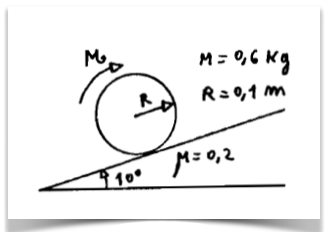
\includegraphics[clip,width = .45\columnwidth]{img/2doparcial2023-0.png}
\end{center}
\end{figure}

\eje{\bf TEMA 6: MOVIMIENTO OSCILATORIO} [EJERCICIO 4 PRÁCTICA 6] Una plataforma realiza un MAS según una dirección vertical con amplitud A = 0.5 m. 

a) ¿Cuál debe ser el período mínimo de oscilación para que un cuerpo colocado sobre la plataforma no se separe de ella? 

b) Luego, ¿qué pasaría si el período fuera aún menor?

\end{document}